\paragraph{Filtered FE velocity and signed shear compositions.}
Nine Fourier orientations are obtained from a projected $P_4$ streamfunction on perturbed triangles. Two smooth periodic profiles are transported to $T=0.5$. Independent RK4 characteristics refine to a foot discrepancy below $5.2\,10^{-14}$. The same FE space and filtered velocity drive a central/upwind DG--RK4 comparator. All evolution operators use CUDA graphs, including the FE observation at every semi-Lagrangian step.
The measured orders between two and four time steps at $n=128$ are 3.97, 4.06, 5.85 for the three-stage fourth-order, five-stage fourth-order and seven-stage sixth-order compositions. These are pre-plateau measurements, not uniform temporal orders at fixed discrete space.
\begin{center}\small\begin{tabular}{lrrr}\toprule Method & Steps & Relative error & Evolution (s)\\\midrule
DG central & 310 & 7.029e-08 & 0.2896\\
DG upwind & 303 & 3.748e-08 & 0.2620\\
Memory/Y6 & 4 & 4.729e-08 & 0.1046\\
Memory/Y6 & 8 & 2.058e-08 & 0.2086\\
Reset/Y6 & 4 & 4.743e-08 & 0.1069\\
Reset/Y6 & 8 & 2.167e-08 & 0.2124\\
\bottomrule\end{tabular}\end{center}
The table reports medians of five blocks with alternating case order, excluding assembly, graph capture and the independent reference. The report provides the full timing ranges. Similar performance of reset and persistent memory would attribute the speed advantage to the transport composition, not to persistent memory. No intermediate reaction is included in this comparison.
\begin{figure}[htbp]\centering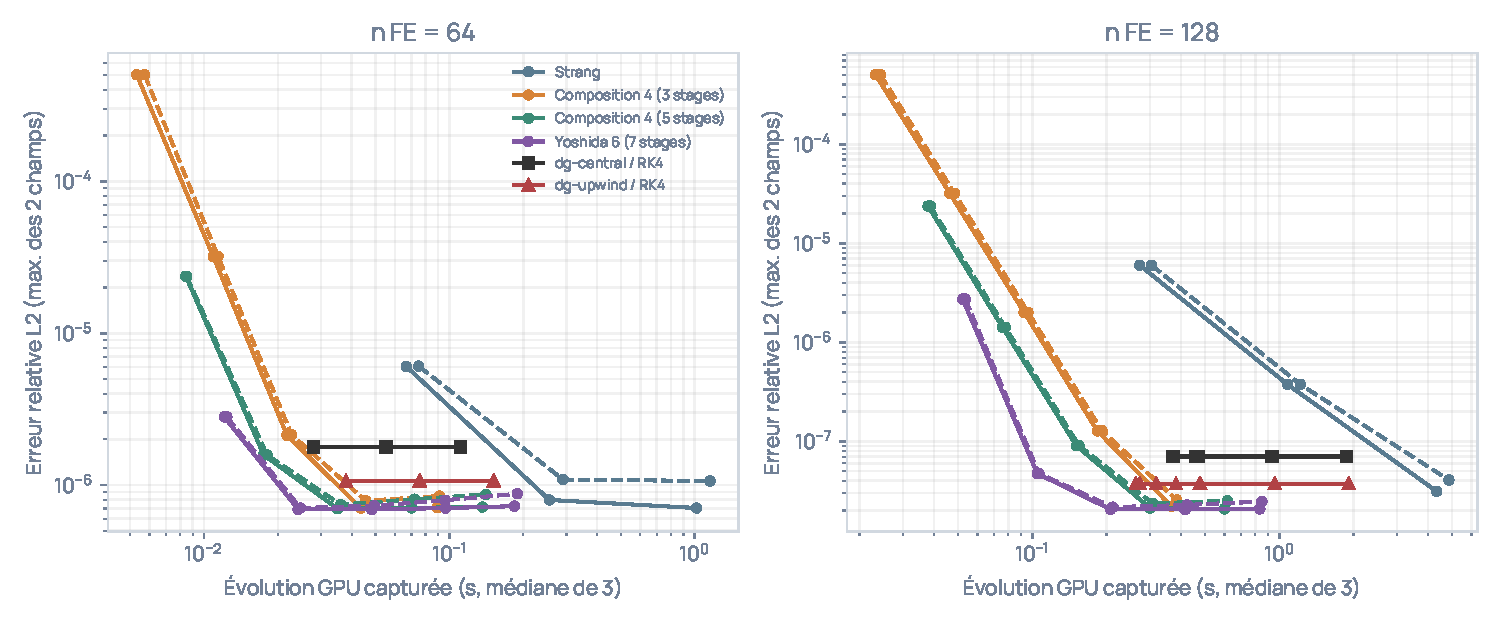
\includegraphics[width=\linewidth]{night-hamiltonian-cost.pdf}
\caption{Accuracy versus evolution cost for identical FE spaces and velocities. Solid lines preserve memory; dashed lines reconstruct it from the FE observation after every step. Preparation costs are excluded.}\end{figure}
A second streamfunction, $0.04\exp(0.7\cos(2\pi(x-0.5))+0.45\cos(2\pi(y-0.5))-1.15)$, has infinitely many Fourier modes. Its FE moments are truncated to a square spectral band and checked against independent analytic-function FFT moments. The reference integrates the original, untruncated analytic velocity.
At spectral radius ten, $n=128$ and eight steps, the maximum component relative error is 2.263e-09, against an FE projection floor 2.197e-09; the sampled relative velocity error is 5.657e-12. This uses 220 retained wavevectors. Increasing the spectral bandwidth substantially increases cost, and this study alone establishes no efficiency advantage for general velocities.
\begin{figure}[htbp]\centering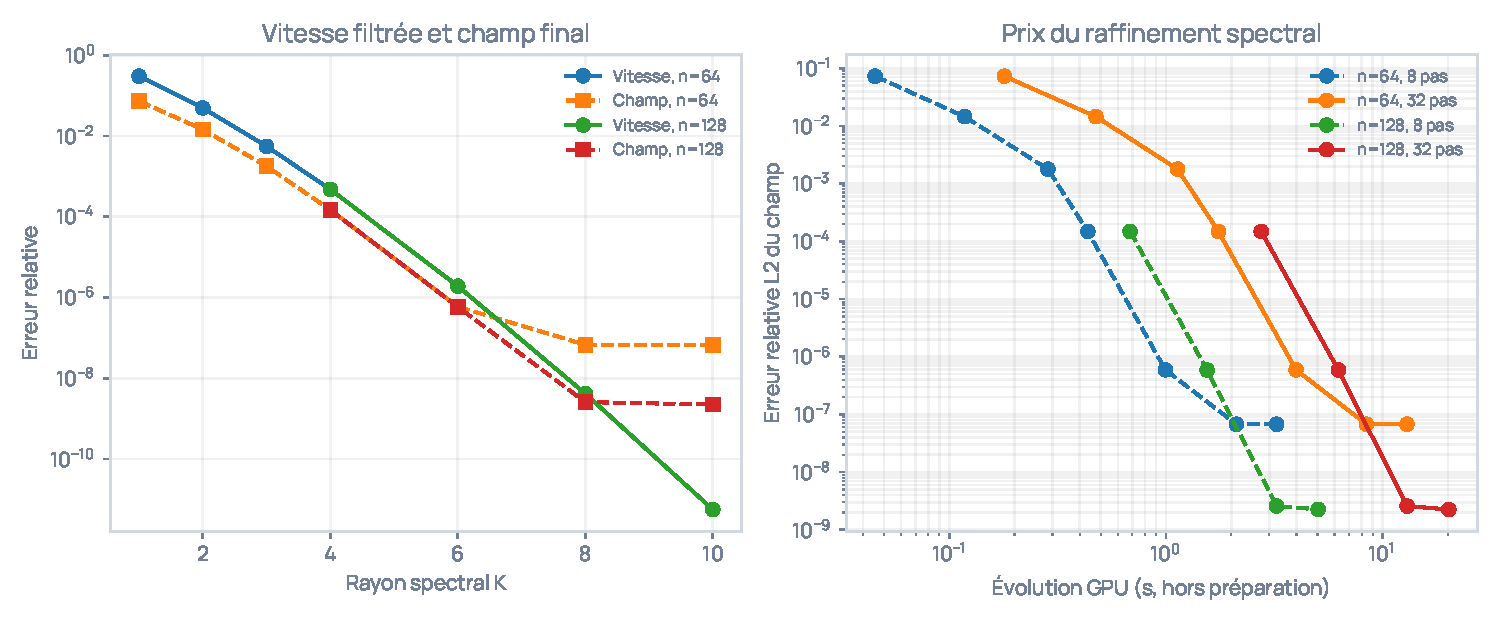
\includegraphics[width=\linewidth]{night-hamiltonian-broad.pdf}
\caption{Spectral truncation of a non-bandlimited FE streamfunction. Analytic characteristics separate velocity filtering from transport error.}\end{figure}
